\documentclass[a4paper, man, natbib, floatsintext]{apa6}
\usepackage[maxfloats=25]{morefloats}
\usepackage{standalone}
\usepackage[english]{babel}
\usepackage[utf8x]{inputenc}
\usepackage{amsmath,amssymb}
\usepackage{graphicx}
\graphicspath{{analyses/code/}{analyses/figures/}}
\usepackage{multicol}
\usepackage{multirow}
\usepackage{booktabs}
\usepackage{url}
\usepackage{rotating}
\usepackage[toc,page]{appendix}
\usepackage{color}
\usepackage{subscript}
\usepackage{threeparttable}
\usepackage{threeparttablex}
\usepackage{longtable}
\usepackage{times}
\usepackage{upgreek}
\usepackage{setspace}
%\AtBeginEnvironment{tabular}{\onehalfspacing}
%% Revision:
%% Use "final" option to remove all tracking markups
\usepackage[dvipsnames]{xcolor}
\usepackage[authormarkup=none]{changes}
\definechangesauthor[name={JJ}, color=blue]{jj}
%%%%%%%%%%%%%%%%%%%%%%%%%%%%%%%%%%%%%%%%%%%%%%%%%%%%%%%%%%%
\title{The influence of sample size on preferences from experience}
\shorttitle{sample size and preference}
\author{Janine Christin Hoffart\\Jana B. Jarecki\\Gilles Dutilh\\J\"org Rieskamp}
\affiliation{University of Basel, Department of Psychology, Center for Economic Psychology}
\leftheader{Hoffart, Jarecki, Rieskamp, Dutilh}

\abstract{People often learn from experience about the distribution of outcomes of risky options. Typically, people draw small samples, when they can actively sample information from risky gambles to make decisions. \added[id=jj]{We examine how the size of the sample that people experience in decision from experience affects their preferences between risky options. In two studies (N=40 each) we manipulated the size of samples that people could experience from risky gambles and measured subjective selling prices and the confidence in selling price judgments after sampling.} The results show that, on average, sample size influenced neither the selling prices nor confidence. However, \added[id=jj]{cognitive modeling of individual-level learning showed that most} participants could be classified as Bayesian learners, whereas the minority adhered to a frequentist learning strategy. The observed selling prices of Bayesian learners changed with sample size as predicted by Bayesian principles, whereas sample size \added[id=jj]{affected} the judgments of frequentist learners \added[id=jj]{much less}. These results illustrate the variability in how people learn from sampled information and provide an explanation for why sample size often does not affect judgments.
}

\keywords{D--E gap, valuations from experience, \added[id=jj]{risky gambles}}
\authornote{This research was supported by a grant (SNSF \# 143854) from the Swiss National Science Foundation to the third and fourth author. We thank Anita Todd for editing the manuscript. 

Correspondence concerning this article should be addressed to Janine Christin Hoffart, University of Basel, Department of Psychology, Missionsstrasse 62a, 4055 Basel, Switzerland.  E-mail: janine.hoffart@unibas.ch}





%%%%%%%%%%%%%%%%%%%%%%%%%%%%%%%%%%%%%%%%%%%%%%%%%%%%%%%%%%%
\begin{document}

\maketitle

In everyday life, people often form preferences on the basis of past experiences. The strength of these preferences arguably depends on the amount of previous experience. Someone who has visited a restaurant for many years and has always had positive experiences likely has a stronger positive preference for this restaurant than someone who visited the restaurant only once and had a positive experience. Thus, even if the relative frequency of positive experiences is similar, the strength of preferences can differ depending on the amount of experience. We examined how people's preferences in an experience-based judgment situation under risk evolve as a function of growing experience. 

%In everyday life people often base their preferences on past experiences. How much experience people have made with an option arguably influences how strong people's opinion about this option is. Someone who had made 50 out of 50 good experiences with a restaurant probably has a stronger preference for this restaurant than someone who had made 1 out of 1 good experience with this restaurant although the relative frequency of good experiences is the same in both situations. Here, we study, how people's preferences (i.e. valuations) in an experience-based task evolve as a function of growing experience. 

\section{Search Effort in Experience-Based Tasks and the Description-Experience Gap}
\added[id=jj]{Search effort refers to the sample size that people draw in experience-based risky choice tasks. In these tasks, people learn about the distribution of outcomes of gambles by repeatedly drawing outcomes from a gamble until they feel confident to make a judgment or decision \citep[e.g.,][]{Hertwig2004, Hau2008}.} By contrast, in description-based tasks, people judge risky gambles from numerical, graphical, or textual summaries of the gambles' outcome distributions. Past research found that risk preferences differ between experience- and description-based tasks (the decision-experience gap or D--E gap). In decisions from description, people choose as if they overweight rare events \citep{Kahneman1979}, in decisions from experience, they choose as if they underweight rare events \citep{Hertwig2004}.

People's search effort (size of the sample they draw) in experience-based tasks plays a key role in explaining the D--E gap, because smaller samples cause higher sampling error. Sampling error means that the observed relative frequency in the outcome sequence deviates from the objective outcome probability \citep{Hadar2009}. Drawing more samples diminishes the sampling error, but usually the number of samples drawn by people are not sufficient to allow inferences about the true distribution of a gamble with a skewed outcome distribution. Participants in \cite{Hertwig2004}, for instance, drew a median of 15 outcomes per decision, and with this number of outcomes, the skew of a two-outcome gamble's binomial sampling distribution implies that more people undersample than oversample low-probability outcomes (rare events). Indeed, averaged across trials, in Hertwig et al.'s study, the rare event was undersampled by $78\%$ of the participants. Other studies have reported similar sampling errors \citep[e.g.,][]{Hau2008,Rakow2008}. Explanations for why people often search insufficiently include limits of memory, opportunity costs \citep{Hau2008}, or adaptive choice simplification \citep{Hertwig2010}: Simulations have shown that small samples amplify the differences between the observed means of the outcome distributions of risky options.

\added[id=jj]{To understand the D--E gap, previous work tried to eliminate sampling error in experienced-based risky decision making.} Attempts have involved encouraging participants to draw larger samples \citep{Hau2008}, showing samples that represent the gambles' true probability distributions \citep{Ungemach2009}, showing large numbers of random samples \citep{Hau2008,Hau2010}, describing gambles to match the outcome distribution sampled by other participants \citep{Rakow2008}, and only analyzing trials in which the drawn sample approximates the gambles' true outcome distribution \citep[e.g.,][]{Camilleri2009, Camilleri2011a}. Sometimes the D--E gap diminished \citep{Hau2008,Hau2010, Ungemach2009} or vanished \citep{Gloeckner2012, Camilleri2009,Camilleri2011a,Rakow2008}, but despite these mixed findings, the D--E gap is a robust phenomenon \citep[for a recent meta-analysis, see][]{Wulff2017}. \added[id=jj]{Most of this research focused on sampling error in combination with sample size, because sampling error is more likely in small samples.}

\added[id=jj]{In the present work we examine the role of sample size in experience-based evaluations independently of sampling error. To do so, we manipulated the number of outcomes drawn from a risky options' outcome distribution (sample size) and elicited people's preferences (i.e., selling prices). Our experimental design eliminates the sampling error, so that we can examine the pure effect of sample size on people's preferences for risky options in an experienced-based task.}

%While the question whether people process information from description differently than information from experience is definitely interesting, here . Instead we will focus on how sample size influences how risky options are evaluated. To do so, we manipulate how many samples people can draw from the options' outcome distributions and study

\section{How Does Sample Size Influence Preferences?}
The question of how sample size influences judgments has interested psychologists for decades \citep[e.g.,][]{Tversky1971, Griffin1992}. We investigate how sample size influences preferences from experience by contrasting two theories: \textit{the belief in the law of small numbers} \citep{Tversky1971} and \textit{Bayesian updating}. 

The belief in the law of small numbers, which was formulated by \cite{Tversky1971}, is people's belief that it is highly probable that a small sequences of random draws represents the true outcome distribution. When asked to mentally produce a short sequence of random coin tosses, people produced sequences with a relative frequency of heads and tails of $.50$ more often than statistically expected \citep{Tversky1971}. In \cite{Griffin1992}, participants ignored sample size in their judgments of coin biases after seeing sequences of coin tosses of different length, some of which were biased. Participants mainly based their estimates of the probabilities associated with the coins on the observed relative frequency of heads and tails. Surprisingly, participants expressed higher confidence in their judgments when the number of coin tosses was small, \added[id=jj]{whereas from a statistical perspective, confidence should be lower for smaller samples.} Several studies have found that people's inferential \citep[e.g.,][]{Kutzner2016}, perceptual \citep[e.g.,][]{Kvam2016}, and preferential judgments \citep[e.g.,][]{Powell2017} are less sensitive to sample sizes than expected by normative models.

In contrast to the belief in the law of small numbers, Bayesian psychological principles suggest that not only the relative frequency of outcomes but also sample size influences judgments. The Bayesian view offers a normative solution to how people deal with sample sizes. People can treat sample size as a measure of uncertainty, knowing that small samples can lead to a biased representation of the true outcome distribution and larger samples to a more veridical description of the true outcome distribution. Consistently, there is some evidence that people treat sample size as a measure of uncertainty, for instance, when they report preferences for consumer goods \citep{DeMartino2017}, make judgments about group differences \citep{Obrecht2010}, or student performance \citep{Fiedler2002}.

\subsection{Cognitive Models and Hypothesis}
To contrast the Bayesian principles with the belief in the law of small numbers in experience-based probability learning we specified two computational learning models. Before introducing the models, it is crucial to recognize that our experimental methods employ predefined sample sizes and representative sequences. In our experiments, participants sampled a \textit{predefined} number of times from a gamble's outcome distribution and evaluated it by indication of the gamble's selling price. Gambles were two-outcome gamble characterized by a gain and a zero-outcome. Individual gambles were presented with different sample sizes and these sample sequences were \textit{representative} of the gamble's true outcome distribution, which allowed us to isolate the effect of sample size without sampling error. For our task the models were formalized as models of learning the probability with which the nonzero gain outcome occurred for the gambles. (Despite this simplification the models can be extended for cases with different types of outcomes).

We follow an expected utility approach. \added[id=jj]{The subjective expected utility of a risky option is given by the sum of the subjective utilities of the outcomes, weighted by the respective probabilities. We represent the subjective utilities of outcomes by a power utility function, defined as $u(g) = g^{\mathrm{\tau}}$, where $g$ is a gain outcome and $\tau$ is a free risk preference parameter. When the outcome probabilities must be learned, as in decisions from experience, the true probabilities are replaced by the decision makers' beliefs about outcome probabilities. We consider two models of learning the outcome probabilities: A relative frequency (RF) model and a Bayesian value updating (BVU) model, that both formalize people's beliefs about the outcome probabilities after observing outcomes, but follow different psychological mechanism to do so.}

\subsubsection{Relative frequency model}

\added[id=jj]{The \textit{relative frequency (RF) model} forms beliefs about probabilities from relative frequencies. It formalizes how people, who trust in the law of small numbers, estimate probabilities.} The model predicts that after $t$ observations, the belief about the probability of a gain outcome corresponds to the observed relative frequencies of gains
$${B}_{\mathrm{RF}, t}  =  \frac{n_t}{t} ,$$
\added[id=jj]{where $n_t$ represents the number of gains observed until sample number $t$ (including $t$).}

\added[id=jj]{The relative frequency model predicts that changes in sample size do not change the resulting valuations of risky options unless the sample size changes the observed relative frequencies. The relative frequency model does not incorporate prior beliefs about the probabilities of outcomes.}

\subsubsection{Bayesian value updating model}
The \emph{Bayesian value updating (BVU)} model implements a Bayesian perspective on probability learning and the resulting uncertainty from sampling. Following Bayesian principles, beliefs about probabilities are based on the observed frequencies and based on prior beliefs about the probabilities of outcomes. The Bayesian model formalizes the distribution of the beliefs about gain probabilities by a beta distribution ${B}_{\mathrm{BVU}} \sim Beta(\alpha,\beta)$ \cite[for an introduction to Bayesian cognitive models, see][]{Griffiths2008a}. The initial beliefs at $t = 0$ are given by a prior belief distribution $B_{\mathrm{BVU},0} \sim Beta(\alpha_0$, $\beta_0)$, with parameters that can be seen as prior pseudo-observations of gains ($\alpha_0$) and zero-outcomes ($\beta_0$). \added[id=jj]{Upon experiencing a sample with size $t$, the learners update their prior belief to a posterior belief $B_t$ represented as}

$$B_{\mathrm{BVU},t} \sim Beta(\alpha_t, \beta_t),$$
$$\text{with } \alpha_t = \alpha_0 + \delta n_t, \text{ and } \beta_t = \beta_0 + \delta n_0,$$

\noindent\added[id=jj]{where $n_t$ represents the number of gain outcomes and $n_0$ represents the number of zero outcomes observed up to outcome number $t$. The parameter $\delta$ is a learning rate that scales the number of observations and can account for individual differences in the revision of prior beliefs \citep{Edwards1967,Tauber2017,Jarecki2017}.  As point estimate of people's (posterior) beliefs about the probability of the gain outcome, we use the expected value of the posterior distribution, which is given by $\frac{\alpha_t}{\alpha_t + \beta_t}$.}

\added[id=jj]{The learning rate adjusts the change in the prior beliefs given new information. Conservative learners ($\delta < 1$) under-weight the incoming observations and revise their prior beliefs less than expected from Bayes' theorem. Liberal learners ($\delta > 1$) overwrite their prior beliefs quicker than the optimal Bayesian learner, characterized by $\delta = 1$. Thus the learning rate governs the degree to which learners revise their prior beliefs about the probabilities of risky outcomes with a new outcome that they learn about.}

The learning process of the Bayesian (BVU) model is illustrated in Figure \ref{fig:sensi}\added[id=jj]{, showing the model's prior and posterior beliefs about the probability of a gain as a function of the sample size and the prior beliefs about the gain probability. The orange curves show different initial beliefs, the purple and black curve illustrate the change in belief after observing a small representative sample of outcomes (\textit{t}$=$5) and a large representative sample (\textit{t}$=$30, with equal relative frequencies in both samples). For large samples, the beliefs approximate the true probability with which the gain occurs for a gamble, independently of the prior belief. In contrast, for small samples, the prior belief changes the models' posterior belief about the gamble's gain probability (purple curve). Unlike the Bayesian model, the relative frequency model predicts a constant $Pr(\text{gain})$ probability equal to the true $Pr(\text{gain})$ probability after the model saw the representative sequence of outcomes, such as 1 gain outcome out of 5 outcomes or 6 gain outcomes out of 30 outcomes.}

\begin{figure}[htbp] 
  \centering
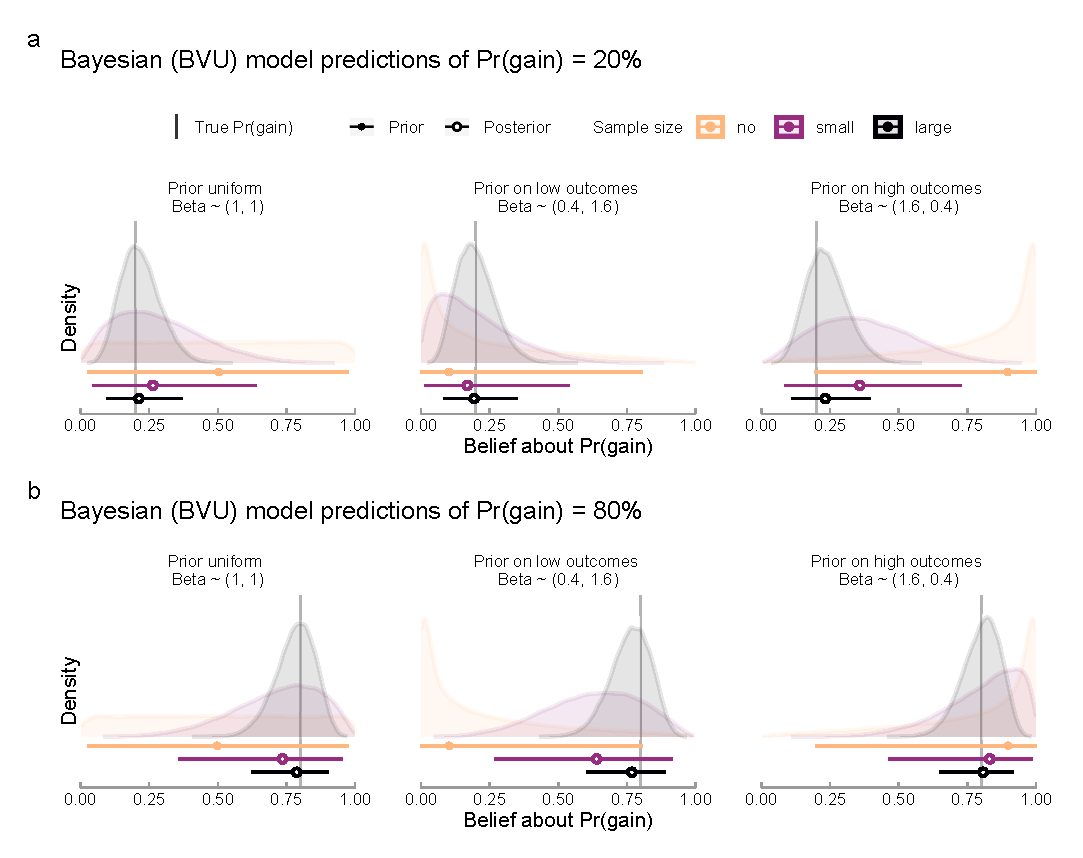
\includegraphics[width=1\linewidth, keepaspectratio]{fig1.eps}
  \caption{\added[id=jj]{\BVU model prediction about probability beliefs depending on different gambles, sample sizes, and prior belief distributions. Predicted beliefs are obtained using $\delta=1$. (a) Beliefs about a gamble with low probability of a gain. Shown are the distribution, mean, and quantile interval of the prior belief and the posterior beliefs after seeing samples of size 5 and 30 (small and large, resp); left, middle, and right panels show model behavior for three types of prior beliefs. (b) Beliefs about a gamble with high probability of a gain.}}
  \label{fig:sensi}
\end{figure}

The Bayesian (BVU) model predicts that people's prior beliefs and the sample size influence their (posterior) valuations. This is because as sample size increases, the beta-distributed belief shifts from the mean of the prior belief in the direction of the true underlying probability of the gain (see Figure \ref{fig:sensi}). Whether the model predicts a decrease or an increase in valuations with growing sample size depends on the shape of the prior belief and the true probability of a gain. In a situation with a true gain probability of less than 50\%, learners with a uniform prior belief or a prior beliefs that a gain is very likely should decrease their valuations as a function of sample size, according to the BVU model. Learners with a prior belief that a gain is very unlikely, however, should increase their valuations as a function of sample size. By contrast, if the true gain probability is larger than 50\%, learners with uniform priors should increase their valuations with sample size, and decrease them when having the prior belief that gains are very likely. In all cases, with increasing sample size the posterior beliefs becomes more and more accurate. Therefore, the model also predicts that confidence in valuations increases with increasing sample size. %We also test this prediction by assessing confidence ratings.

\deleted[id=jj]{Following \cite{Griffin1992}, we also asked participants for their confidence in their valuations. We tested whether people would be more confident about their responses when the sample size was small, as found by \cite{Griffin1992}.}

\section{Study 1}
In Study 1, we aimed to measure the preference strength for risky options, and therefore, we prompted participants to evaluate individual gambles \citep[similer to e.g.,][]{Ashby2014, Golan2014, Pachur2012}, because evaluations allow us to measure preference strength more precisely than binary choices between gambles. This is important, as detecting subtle differences in strength of preference requires fine-grained measurement scales. \added[id=jj]{Following \cite{Griffin1992}, we also asked participants for their confidence in their valuations to test if confidence were higher in small samples as found by \cite{Griffin1992}.} Second, we aimed to lay bare the precise effects of sample size---therefore, we presented each gamble with various sample sizes. \added[id=jj]{We presented representative samples, which eliminates sampling error and allows} for an unbiased comparison of sample size effects. The order of outcomes within a sampling sequence was random. \added[id=jj]{A third, but sub-ordinate, goal was comparing valuations from experience with valuations from description.} Therefore, we added a block where people made valuations from description. However, as our main goals involved studying how preferences change as a function of sample size, we refrained from manipulating the order of the experience and description blocks. All people made valuations first from experience and afterward in a separate block from description. 

In Study 1, we examined how people form valuations from experience when they know the possible outcomes before they start sampling. In a situation where the outcomes are known, learning is simplified because participants only need to learn the outcome probabilities from experience. 

\subsection{Method}
\subsubsection{Participants}
Forty people (31 women, 9 men) from the participant pool of the University of Basel between 18 and 40 years old ($M = 23.41$ years, $SD = 4.86$) participated in the study. Participants could choose between a show-up fee of 10 CHF (approximately \$11.10 at the time of the experiment) or course credit. Additionally, each participant received a bonus payment that depended on the outcome of a randomly selected trial ($M = \$6.38$, $SD = \$7.62$).

\subsubsection{Stimuli and Design}
\added[id=jj]{The design was a within-subject design, participants evaluated two-outcome gambles from experience and from description. Six gambles with either a gain or a zero outcome were created by crossing two gamble types (\textit{\$-bet}, \textit{p-bet}) with three expected values (2.00, 3.20, 4.00), see Table \ref{table:Lotteries}. Three gambles offered a high gain with low probability (\$-bet), and three offered a small gain with high probability (p-bet, notation following \citealp{Lichtenstein1971}). In the experience-based valuation each gamble was crossed with four sample sizes: extra small, small, medium, large (xs, s, m, l), listed in Table \ref{table:Lotteries}. As shown in Table~ \ref{table:Lotteries} the extra small sample size (xs) consisted of a sample size of 5, 6, or 7 outcomes, which allowed us to represent rare events of 1/5, 1/6, and 1/7 (20\%,  17\%, 14\%, respectively). The small sample size equaled xs $\times$ 2, the medium sample size equaled xs $\times$ 3, and the large sample size equaled xs $\times$ 6. Participants saw each gamble with each of the four sample sizes three times in fully randomized order (each gamble was seen 12 times).}

To avoid memory effects between trials, 18 filler trials were shown\deleted[id=jj]{that involved six gambles with outcomes identical to Table~\ref{table:Lotteries}, but probabilities changed to 75\% (\$-bets) and 25\% (p-bets). The filler gambles' sample sizes were 4, 8, and 16. Filler trials were excluded from analyses, because they only aimed at minimizing memory-effects.}\footnote{Filler trials involved six gambles with outcomes identical to Table~\ref{table:Lotteries}, but probabilities changed to 75\% (\$-bets) and 25\% (p-bets). The filler gambles' sample sizes were 4, 8, and 16.} Filler trials were excluded from analyses, because they only aimed at minimizing memory-effects.

\begin{table}[bth]
\begin{center}
\begin{threeparttable}
\caption{Gambles and Sample Sizes Used in Studies 1 and 2\label{table:Lotteries}}
\begin{tabular}{llccccccc}
\toprule
 &  &  &  &  & \multicolumn{4}{c}{Sample Size} \\
\cmidrule(r){6-9}
Gamble ID & Type & X & Pr & EV & xs & s & m & l\\
\midrule
1 & \$-bet & 16.00 & 0.20 & 3.20 & 5 & 10 & 15 & 30\\
2 & \$-bet & 12.00 & 0.17 & 2.00 & 6 & 12 & 18 & 36\\
3 & \$-bet & 28.00 & 0.14 & 4.00 & 7 & 14 & 21 & 42\\
4 & p-bet & 4.00 & 0.80 & 3.20 & 5 & 10 & 15 & 30\\
5 & p-bet & 2.40 & 0.83 & 2.00 & 6 & 12 & 18 & 36\\
6 & p-bet & 4.70 & 0.86 & 4.03 & 7 & 14 & 21 & 42\\
\bottomrule
\addlinespace
\end{tabular}
\begin{tablenotes}[para]
\normalsize{\textit{Note.} \textit{X} = gain in Swiss Fr., \textit{Pr} = probability of gain, \textit{EV} = expected value, \textit{Sample Size} = total number of observations in the experience condition categorized as \textit{xs} = extra small, \textit{s} = small, \textit{m} = medium, \textit{l} = large. The probability is expressed as the ratio of the relative frequency of the number of gain observations to the number of observations in the smallest sample size category (xs) of this gamble, namely 1/5, 1/6, 1/7, 4/5, 5/6, and 6/7 for gamble IDs 1 through 6, respectively.}
\end{tablenotes}
\end{threeparttable}
\end{center}
\end{table}

After the experience block, participants saw each gamble three times in a description format. In this block, participants received a description of the gamble's outcome and the associated probability; probabilities were rounded to one decimal place (1/5 = 20\%, 1/6 = 16.7\%, 1/7 = 14.3\%). Again, presentation order of all trials was fully randomized.


\subsubsection{Procedure}
Participants read printed instructions and completed a questionnaire that ensured their understanding of the instructions; the experimental task was computerized. \added[id=jj]{Participants judged the value of the risky gambles (see Table~\ref{table:Lotteries}) and rated the confidence in their judgments. Gambles were judged one-by-one, in the experience-based format given different sample sizes, followed by the description format. In the experience format, participants were informed about the outcomes but not the outcome probabilities of a gamble, which they learned by repeatedly sampling outcomes. The possible outcomes were represented by numbers in a circle (gains were in a black circle, zero-outcomes white) and stayed on screen throughout sampling. Pressing the space bar sampled an outcome; the realized outcome appeared as a black or white circle for 250 ms; sampling ended after a predefined sample size (listed in Table~\ref{table:Lotteries}). Participants were informed a priori about the pre-specification of the sample size. The sampled outcomes were representative for the gambles (for example, drawing a sample of size 5 from a gamble with $Pr(\text{gain})=20\%$ resulted in one gain outcome and four zero outcomes). After sampling, participants evaluated the gamble and rated their confidence, and proceeded to the next trial. Sample size changed from trial to trial.} The trial order and outcome sequence within a trial was randomized for individual participants. \deleted[id=jj]{After participants had drawn the required number of outcomes, they were prompted for (1) their valuation of the gamble (see below) and (2) their confidence in their valuation} 

Confidence was measured on a 7-point Likert scale (from 0 = \textit{very unconfident} to 6 = \textit{very confident}). Valuations of gambles were measured as selling prices following the Becker--DeGroot--Marschak (BDM) method \citep{Becker1964}: \deleted[id=jj]{For each gamble}Participants stated their selling prices in terms of the lowest monetary amount for which they would give up the right to gamble. Prices could range from 0.00 to the current gain in CHF, with increments of 0.10 CHF. The BDM auction was incentivized as follows. The selling price that a participant entered was compared to a random value drawn from all possible selling prices in the trial. If this random number was larger than the stated selling price, the participant ``sold'' the gamble and received a monetary amount \replaced[id=jj]{that equaled}{equal to} the random number. If the random number was equal to or smaller than the selling price, the participant got to gamble. For the BDM, the optimal strategy is always to report the true selling price.\footnote{\label{logic.BDM}
To understand this logic, consider the following example: A person has a true selling price for a given gamble of \$3. If this person sets her selling price too low (e.g., \$2) and the randomly generated number is \$2.10, she sells her gamble for a lower price than her true selling price. If, however, she sets her selling price too high (e.g., \$5) and the randomly generated number is \$4, she keeps and plays her gamble, although she actually would have preferred to receive the \$4.
} \added[id=jj]{Detailed instructions as well as an example of the BDM auction were presented to the participants to explain the auction's mechanism. We used a short questionnaire to ensure that all participants had understood how the auction worked.}

\subsection{Results}
\added[id=jj]{The analyses were conducted in statistical software R version 6.0.1 \citep{R} using the BayesFactor package version 0.9.12 \citep{BayesFactor}; inferences were based on the Bayes factor ($BF\textsubscript{ij}$).}\footnote{Bayes factors quantify how much more or less likely the data are under Model i ($\mathrm{M}\textsubscript{i}$) than Model j ($\mathrm{M}\textsubscript{j}$). A Bayes factor of 1 ($BF\textsubscript{ij} = 1$) means that the data do not discriminate between the two models $\mathrm{M}\textsubscript{i}$ and $\mathrm{M}\textsubscript{j}$. A Bayes factor of 5 (i.e., $BF\textsubscript{ij} = 5$) means that the data are 5 times more likely under $\mathrm{M}\textsubscript{i}$ than under $\mathrm{M}\textsubscript{j}$. A Bayes factor of $1/5$ ($BF\textsubscript{ij} = 1/5$) means that the data are 5 times more likely under $\mathrm{M}\textsubscript{j}$ (note that $BF\textsubscript{ji} = 1/BF\textsubscript{ij}$).} 

\documentclass[a4paper, man, floatsintext]{apa6}
\usepackage{lmodern}
\usepackage{amssymb,amsmath}
\usepackage{ifxetex,ifluatex}
\usepackage{fixltx2e} % provides \textsubscript
\ifnum 0\ifxetex 1\fi\ifluatex 1\fi=0 % if pdftex
  \usepackage[T1]{fontenc}
  \usepackage[utf8]{inputenc}
\else % if luatex or xelatex
  \ifxetex
    \usepackage{mathspec}
  \else
    \usepackage{fontspec}
  \fi
  \defaultfontfeatures{Ligatures=TeX,Scale=MatchLowercase}
\fi
% use upquote if available, for straight quotes in verbatim environments
\IfFileExists{upquote.sty}{\usepackage{upquote}}{}
% use microtype if available
\IfFileExists{microtype.sty}{%
\usepackage{microtype}
\UseMicrotypeSet[protrusion]{basicmath} % disable protrusion for tt fonts
}{}
\usepackage{hyperref}
\hypersetup{unicode=true,
            pdfauthor={Jana B. Jarecki},
            pdfborder={0 0 0},
            breaklinks=true}
\urlstyle{same}  % don't use monospace font for urls
\usepackage{graphicx,grffile}
\makeatletter
\def\maxwidth{\ifdim\Gin@nat@width>\linewidth\linewidth\else\Gin@nat@width\fi}
\def\maxheight{\ifdim\Gin@nat@height>\textheight\textheight\else\Gin@nat@height\fi}
\makeatother
% Scale images if necessary, so that they will not overflow the page
% margins by default, and it is still possible to overwrite the defaults
% using explicit options in \includegraphics[width, height, ...]{}
\setkeys{Gin}{width=\maxwidth,height=\maxheight,keepaspectratio}
\IfFileExists{parskip.sty}{%
\usepackage{parskip}
}{% else
\setlength{\parindent}{0pt}
\setlength{\parskip}{6pt plus 2pt minus 1pt}
}
\setlength{\emergencystretch}{3em}  % prevent overfull lines
\providecommand{\tightlist}{%
  \setlength{\itemsep}{0pt}\setlength{\parskip}{0pt}}
\setcounter{secnumdepth}{0}
% Redefines (sub)paragraphs to behave more like sections
\ifx\paragraph\undefined\else
\let\oldparagraph\paragraph
\renewcommand{\paragraph}[1]{\oldparagraph{#1}\mbox{}}
\fi
\ifx\subparagraph\undefined\else
\let\oldsubparagraph\subparagraph
\renewcommand{\subparagraph}[1]{\oldsubparagraph{#1}\mbox{}}
\fi

%%% Use protect on footnotes to avoid problems with footnotes in titles
\let\rmarkdownfootnote\footnote%
\def\footnote{\protect\rmarkdownfootnote}

%%% Change title format to be more compact
\usepackage{titling}

% Create subtitle command for use in maketitle
\providecommand{\subtitle}[1]{
  \posttitle{
    \begin{center}\large#1\end{center}
    }
}

\setlength{\droptitle}{-2em}

  \title{}
    \pretitle{\vspace{\droptitle}}
  \posttitle{}
    \author{Jana B. Jarecki}
    \preauthor{\centering\large\emph}
  \postauthor{\par}
      \predate{\centering\large\emph}
  \postdate{\par}
    \date{20 November, 2019}

\usepackage{natbib} \usepackage{threeparttable} \usepackage{booktabs}
\shorttitle{test} \usepackage{setspace}
\AtBeginEnvironment{tabular}{\singlespacing} \usepackage{times}
\usepackage{changes} \definechangesauthor[name={JJ}, color=orange]{jj}
\usepackage{upgreek} \AtBeginDocument{\let\maketitle\relax}

\begin{document}

\subsubsection{Evaluations of gambles and sample sizes}

Table \ref{tab:means_study1} summarizes the evaluations of the gambles
by format (description vs.~experience) and sample size (xs, s, m, l).
For instance, across sample sizes xs, s, m, and l, our participants
evaluated gamble 4 with an average of \(2.80, 2.91, 2.80, 2.95, 3.08\)
(respectively). Across gambles, the evaluations were not influenced by
sample sizes, which a model comparison among analyses of variance
(ANOVA) of the judgments confirmed: an ANOVA with the predictors gamble
type and gamble expected value (Model 0) outperformed models with the
additional predictors sample size (\(BF_{01}= 396\)) and a sample-size x
gamble-type interaction (\(BF_{02} > 1000\), all models had
by-participant random effects). The \$-bet gambles were evaluated higher
(\(M=5.78, SD=3.94\)) than the p-bet gambles (\(M=2.74, SD=1.09\)),
although the \$-bets and p-bets had the same expected values,
\(BF > 1000\) in favor of an ANOVA that predicts evaluations as a
function of gamble type over an ANOVA without the predictor gamble type
(both models include by-participant and by-expected-value random
effects).

The evaluations in the experience condition were not driven by primacy
or recency: neither the outcomes that participants sampled in the first
half of the sampling phase nor those sampled during the second half of
said phase predict the observed evaluations. A linear model of the
evaluations with the predictor gamble type
(\(\mathrm{M}\textsubscript{0}\)) outperformed a model with the
additional predictor mean of the first half of samples
(\(BF\textsubscript{01} = 16.6\)) and a model with the additional
predictor mean of the second half of samples
(\(BF\textsubscript{02} = 6.7\))

\textit{Description versus experience} That valuations from description
and experience differed for most of the gambles and sample sizes (see
Table \ref{tab:means_study1}, rightmost column). Participants evaluted
experience-based \$-bets higher than described \$-bets, but evaluated
experience-based p-bets lower than described p-bets. ö. In particular,
participants (Gambles 4--6). Thus, we found a D--E gap that is the
opposite of the classic D--E gap observed in choice paradigms. In our
study, participants valued gambles as if they overweighted rare events
from description \textit{and} experience. This effect was even stronger
when people made valuations from experience.

\begin{table}[tbp]

\begin{center}
\begin{threeparttable}

\caption{\label{tab:means_study1}Valuations of Gambles in Study 1}

\begin{tabular}{lccccrr}
\toprule
Condition & Sample size category & Sample size & \textit{Med} & \textit{M} & D--E & D--E:$BF\textsubscript{10}$\\
\midrule
Gamble ID 1 (\$-bet) &  &  &  &  &  & \\
\ \ \ E & xs & 5 & 5.00 & 5.16 & -0.56 & 4\\
\ \ \ E & s & 10 & 4.55 & 5.30 & -0.70 & 64\\
\ \ \ E & m & 15 & 5.00 & 5.34 & -0.74 & 23\\
\ \ \ E & l & 30 & 5.00 & 5.29 & -0.69 & 158\\
\ \ \ D & -- & -- & 4.00 & 4.60 & -- & --\\
Gamble ID 2 (\$-bet) &  &  &  &  &  & \\
\ \ \ E & xs & 6 & 4.00 & 4.33 & -0.71 & 132\\
\ \ \ E & s & 12 & 4.00 & 4.31 & -0.69 & 620\\
\ \ \ E & m & 18 & 4.00 & 4.04 & -0.43 & 4\\
\ \ \ E & l & 36 & 4.00 & 3.99 & -0.37 & 2\\
\ \ \ D & -- & -- & 3.00 & 3.61 & -- & --\\
Gamble ID 3 (\$-bet) &  &  &  &  &  & \\
\ \ \ E & xs & 7 & 6.00 & 7.56 & -0.99 & 4\\
\ \ \ E & s & 14 & 6.70 & 8.40 & -1.83 & 902\\
\ \ \ E & m & 21 & 6.20 & 7.92 & -1.35 & 138\\
\ \ \ E & l & 42 & 6.00 & 7.68 & -1.11 & 15\\
\ \ \ D & -- & -- & 5.00 & 6.57 & -- & --\\
Gamble ID 4 (p-bet) &  &  &  &  &  & \\
\ \ \ E & xs & 5 & 3.00 & 2.80 & 0.28 & >1000\\
\ \ \ E & s & 10 & 3.20 & 2.91 & 0.16 & 3\\
\ \ \ E & m & 15 & 3.00 & 2.80 & 0.28 & 56\\
\ \ \ E & l & 30 & 3.00 & 2.95 & 0.13 & 1\\
\ \ \ D & -- & -- & 3.20 & 3.08 & -- & --\\
Gamble ID 5 (p-bet) &  &  &  &  &  & \\
\ \ \ E & xs & 6 & 2.00 & 1.77 & 0.10 & 8\\
\ \ \ E & s & 12 & 2.00 & 1.75 & 0.12 & 15\\
\ \ \ E & m & 18 & 2.00 & 1.73 & 0.14 & 28\\
\ \ \ E & l & 36 & 2.00 & 1.81 & 0.06 & 1\\
\ \ \ D & -- & -- & 2.00 & 1.87 & -- & --\\
Gamble ID 6 (p-bet) &  &  &  &  &  & \\
\ \ \ E & xs & 7 & 4.00 & 3.46 & 0.18 & 3\\
\ \ \ E & s & 14 & 4.00 & 3.55 & 0.09 & 0\\
\ \ \ E & m & 21 & 4.00 & 3.58 & 0.06 & 0\\
\ \ \ E & l & 42 & 4.00 & 3.70 & -0.06 & 0\\
\ \ \ D & -- & -- & 4.00 & 3.64 & -- & --\\
\bottomrule
\addlinespace
\end{tabular}

\begin{tablenotes}[para]
\normalsize{\textit{Note.} \textit{M} = mean, \textit{Med} = median, D--E = difference between mean description-based valuations and experience-based valuations, $BF\textsubscript{10}$ = Bayes Factor quantifying the evidence for a linear model $\mathrm{M}\textsubscript{1}$ predicting that valuations differ between description and experience over a linear model $\mathrm{M}\textsubscript{0}$ predicting no such differences; both models models contain a by-participant random effect. Gambles IDs 1, 2, and 3 are \$-bets; Gamble IDs 4, 5, and 6 are p-bets.}
\end{tablenotes}

\end{threeparttable}
\end{center}

\end{table}

Although at the aggregate level, sample size does not influence the
evaluations of gambles in our decision from experience paradigm, the
cognitive modeling analyses will show a more nuanced picture.

\subsubsection{Cognitive modeling}

We used computational modeling to analyze the role of sample size in
value judgments more closely, comparing the performance of the
\added[id=jj]{relative frequency} (RF) model and the
\added[id=jj]{Bayesian value updating} (BVU) model.
\added[id=jj]{The models were compared to a baseline model, which predicts a constant evaluation equal to the mean individual evaluation (sensible models are expected to outperform this baseline model).}

\textit{Modeling Procedure.} To fit the model parameters, the observed
and predicted evaluations were normalized to a common range between 0
and 1 (by division through the gain of the presented gamble). Maximum
likelihood was used to estimate the free model parameters at the
participant level, assuming that observations follow a truncated normal
distribution around the model predictions (truncation between 0 and 1)
with a constant standard deviation (\(\sigma\)), that was estimated by
participant (\(0 < \sigma \leq 1\)).
\added[id=jj]{Therefore, the relative frequency model has two free parameters, $\sigma$ and the power utility exponent $\alpha$ ($0 \leq \alpha \leq 20$). The Bayesian value updating model has four free parameters, the gain prior $\theta_G$ ($0 \leq \theta_G \leq 2$), the learning rate $\delta$ ($0 \leq \delta \leq 10$), $\alpha$ and $\sigma$, with the prior on zero outcomes constrained to $\theta_0=2-\theta_G$. The baseline model had two free parameters, the mean evaluation $\mu$ and $\sigma$. We estimated the parameters using an augmented Lagrange multiplier method \citep[Rsolnp package, version 1.16]{Ghalanos2015}. Models were compared based on evidence strength and BIC weights from the Bayesian information criterion (BIC) \cite[evidence in favor of a model compared to the individually best-fitting model][]{Kass1995, Lewandowsky2011}. Higher weights indicate stronger evidence for a model.}

We will first outline the quantitative model fit, followed by the
qualitative model fit, and lastly analyze the effects of sample size
given the cognitive strategies.

\textit{Quantitative Model Fit.} The Bayesian value updating model
described the majority of the participants best (30 of 40; 75\%). The
relative frequency model described 9 participants best (22\%); the
baseline model described only 1 participants best. Figure \ref{fig:fig2}
shows the evidence strength for the models by participant. The models'
mean Bayesian information criterion across all participants equaled
BIC\textsubscript{BVU}\(= -124\), BIC\textsubscript{RF}\(= -110\), and
BIC\textsubscript{BASE}\(= -17\) (lower values indicate better fit).

\begin{figure}[htb]

{\centering 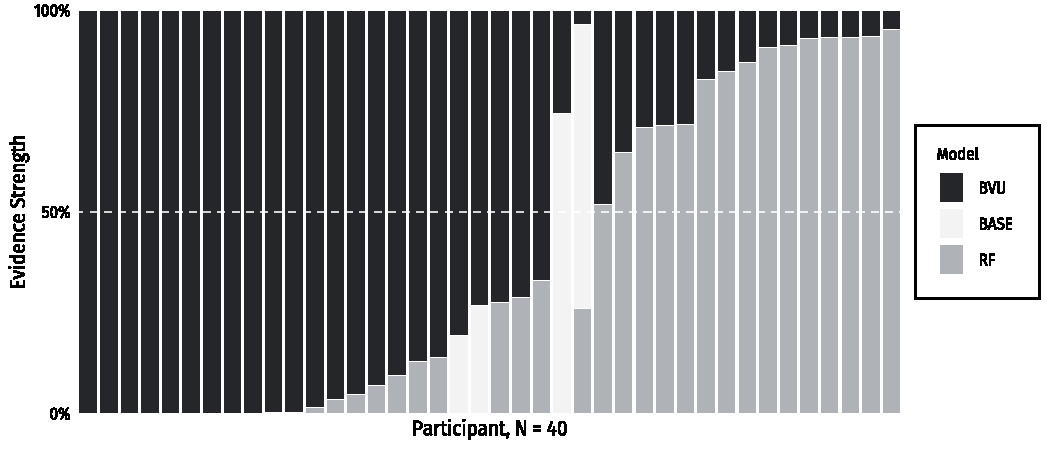
\includegraphics[width=.9\linewidth]{../figures/fig2-1} 

}

\caption{Evidence for the models for individual participants. \textit{RF}$=$ relative frequency model, \textit{BVU}$=$ Bayesian value updating model, \textit{BASE}$=$ Baseline model.}\label{fig:fig2}
\end{figure}

\added[id=jj]{
The estimated parameter of the best-fitting models, which Table \ref{tab:study1_parameter} summarizes, reveal that the power utility exponent ($\alpha$) did not differ for the participants that were described by a Bayesian value updating strategy ($M_{\alpha}= 1.49$) and those using a relative frequency strategy ($M_{\alpha}=1.61$), $\Delta$ $M = -0.08$ 95\% HDI $[-1.01$, $0.74]$, $\mathrm{BF}_{\textrm{01}} = 2.76$. Participants using the Bayesian strategy had, on average, a prior belief that gains occur with 46\% (gain prior $\theta_G = 0.92$; zero-outcome prior $\theta_0 = 1.08$). Also, their estimated learning rate $\delta$ was anti-conservative ($M_{\delta}=1.36$; values $>$ 1 are liberal, 1 is optimal Bayesian, $<$ 1 is conservative learning). The liberal learning rate is unusual given that previous work has found conservative learning \citep{Edwards1967,Tauber2017}. The liberal learning in our data can be explained by that participants repeatedly sampled from the same set of gambles.
}

\begin{table}[tbp]

\begin{center}
\begin{threeparttable}

\caption{\label{tab:study1_parameter}Parameter Estimates of Winning Models, \textit{M (SD)}}

\begin{tabular}{lccccc}
\toprule
Winning Model & $\alpha$ & $\delta$ & $\theta_G$ & $\mu$ & $\sigma$\\
\midrule
BVU (\textit{n}$=$30) & 1.49 (1.47) & 1.36 (2.12) & 0.92 (0.66) & -- & 0.13 (0.07)\\
RF (\textit{n}$=$9) & 1.61 (0.58) & -- & -- & -- & 0.12 (0.02)\\
BASE (\textit{n}$=$1) & -- & -- & -- & 0.47 (NA) & 0.30 (NA)\\
\bottomrule
\addlinespace
\end{tabular}

\begin{tablenotes}[para]
\normalsize{\textit{Note.} \textit{BVU}$=$ Bayesian value updating model, \textit{RF}$=$ relative frequency model, \textit{BASE}$=$baseline model. Parameters denote: $\alpha=$ power utility exponent, $\theta_G$ gain prior, $\mu=$ mean evaluation, $\sigma$ standard deviation.}
\end{tablenotes}

\end{threeparttable}
\end{center}

\end{table}

\textit{Qualitative Model Fit.} The qualitative fit between the models
and the data is shown in Figure \ref{fig:fig5}, which plots the
predictions of the best-fitting models against the observed evaluations
by participant. The models generally describe the data well
\added[id=jj]{($M r\textsubscript{pred,obs} = 0.71$), except in four cases, where even the winning model fails to resemble the data qualitatively (participants s05, s19, s24, s38, with $r\textsubscript{pred,obs} < 0.40$).}
For these cases, for whom the winning model is the Bayesian updating
model, the model must be rejected because of qualitative
mis-fit.\footnote{As robustness check we repeated the model comparison with subjective probability weighting, using Prelec’s single parameter weighting function. This weighting function incorporates non-linearities in the perception of probabilities. However, the quantitative results of the probability weighting model and the utility model, we favored a utility model without probability weighting.}

\begin{figure}[htb]

{\centering 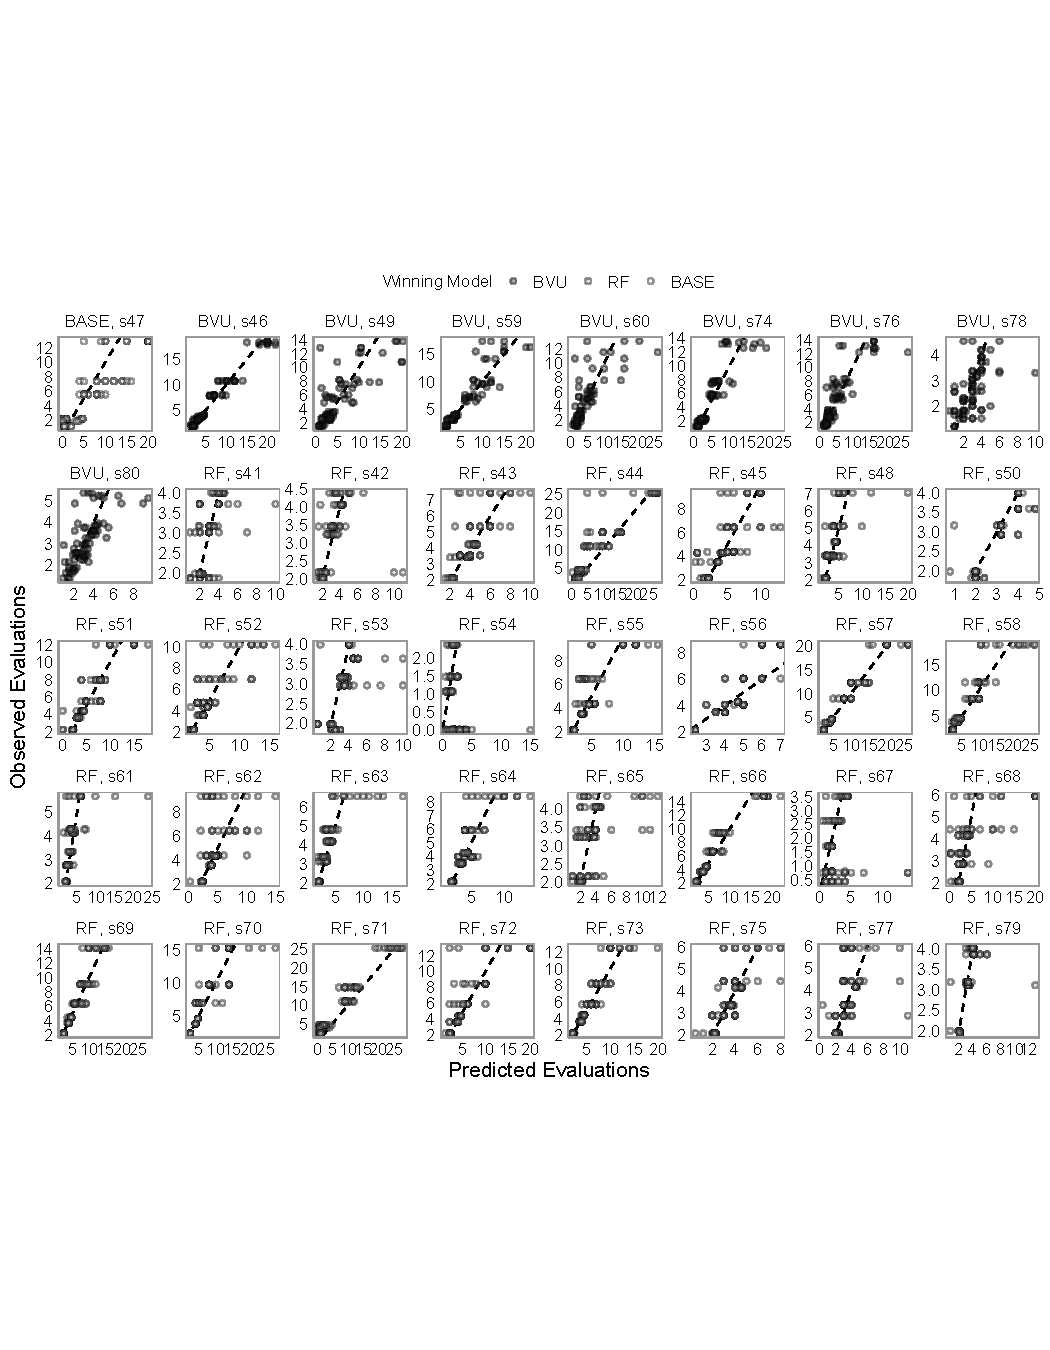
\includegraphics[width=\textwidth]{../figures/fig5-1} 

}

\caption{Predicted evaluations from the best-fitting models plotted against the observed evaluations (by participant). \textit{BVU}$=$ Bayesian value updating model, \textit{RF}$=$ relative frequency model, \textit{BASE}$=$baseline model.}\label{fig:fig5}
\end{figure}

\added[id=jj]{
The cognitive modeling results thus show that most participants were described by a Bayesian strategy, and a minority by a relative-frequency strategy. This strategy heterogeneity helps understanding the behavioral null finding---that sample size seemed to have no effect on valuations---that were observed at the aggregate level (Table \ref{tab:means_study1}). The aggregate analysis fails to take the individual differences in learning strategies into account, while participants are best described by a mixture of strategies. Moreover, the aggregate analysis also fails to account for differences in the prior beliefs about gain probabilities.
}


\end{document}

\clearpage

\subsection{Discussion of Study 1}

Study 1 shows that the size of the sample overall did not have an effect on valuations from experience. \added[id=jj]{Cognitive modeling revealed that the majority of participants were best described by a model following Bayesian principles which treats sample size as a measure of uncertainty. However, a minority of participants were best modelled with a relative frequency strategy that disregards sample size.} Valuations also differed when made from description versus experience. Interestingly, this difference is the opposite of the classic D--E gap that has been reported in choice paradigms: We found evidence that people behaved as if they overweighted rare events when making valuations from description \textit{and} experience. Notably, this overweighting of rare events was even stronger for the experience condition. Importantly, people assigned higher valuations to \$-bets (i.e., gambles that provide a high reward with low probability) than p-bets (i.e., gambles that provide a small reward with low probability) even although both gambles had similar expected values. This finding is in line with recent research that suggested people overweight extreme outcomes in experience-based tasks \citep{Ludvig2017}.

\section{Study 2}
In Study 1 participants knew the possible outcomes before drawing outcomes, which differs from typical decisions from experience paradigms, in which people learn about the outcome values by sampling. To bring our method more in line with the \replaced[id=jj]{standard decision from experience paradigm}{this}, in Study 2 we changed the experimental method such that one outcome had to be learned during sampling.

\subsection{Methods}
The procedure an methods of Study~2 were similar to Study~1. The only difference consisted in that before participants started sampling, they were now only informed about gambles being two-outcome gambles and that one of the outcomes was zero. Unlike in Study 1, the gain amounts of the gambles were not displayed on screen before or during the sampling stage.

\subsection{Participants}
Forty people (38 women, 2 men) between 18 and 27 years old ($M = 21.1$ years, $SD = 2.05$), recruited from the subject pool of the University of Basel, participated. We followed the incentive scheme of Study 1. On average, participants earned a bonus of 7.16 CHF ($SD = 6.91$ at the time of the study). For the data analysis, we compared the same statistical models as described in Study 1.

\subsection{Results}
As before, the analyses were conducted in the software R, models were estimated as in Study 1.

\documentclass[a4paper, man, floatsintext]{apa6}
\usepackage{lmodern}
\usepackage{amssymb,amsmath}
\usepackage{ifxetex,ifluatex}
\usepackage{fixltx2e} % provides \textsubscript
\ifnum 0\ifxetex 1\fi\ifluatex 1\fi=0 % if pdftex
  \usepackage[T1]{fontenc}
  \usepackage[utf8]{inputenc}
\else % if luatex or xelatex
  \ifxetex
    \usepackage{mathspec}
  \else
    \usepackage{fontspec}
  \fi
  \defaultfontfeatures{Ligatures=TeX,Scale=MatchLowercase}
\fi
% use upquote if available, for straight quotes in verbatim environments
\IfFileExists{upquote.sty}{\usepackage{upquote}}{}
% use microtype if available
\IfFileExists{microtype.sty}{%
\usepackage{microtype}
\UseMicrotypeSet[protrusion]{basicmath} % disable protrusion for tt fonts
}{}
\usepackage{hyperref}
\hypersetup{unicode=true,
            pdfauthor={Jana B. Jarecki},
            pdfborder={0 0 0},
            breaklinks=true}
\urlstyle{same}  % don't use monospace font for urls
\usepackage{graphicx,grffile}
\makeatletter
\def\maxwidth{\ifdim\Gin@nat@width>\linewidth\linewidth\else\Gin@nat@width\fi}
\def\maxheight{\ifdim\Gin@nat@height>\textheight\textheight\else\Gin@nat@height\fi}
\makeatother
% Scale images if necessary, so that they will not overflow the page
% margins by default, and it is still possible to overwrite the defaults
% using explicit options in \includegraphics[width, height, ...]{}
\setkeys{Gin}{width=\maxwidth,height=\maxheight,keepaspectratio}
\IfFileExists{parskip.sty}{%
\usepackage{parskip}
}{% else
\setlength{\parindent}{0pt}
\setlength{\parskip}{6pt plus 2pt minus 1pt}
}
\setlength{\emergencystretch}{3em}  % prevent overfull lines
\providecommand{\tightlist}{%
  \setlength{\itemsep}{0pt}\setlength{\parskip}{0pt}}
\setcounter{secnumdepth}{0}
% Redefines (sub)paragraphs to behave more like sections
\ifx\paragraph\undefined\else
\let\oldparagraph\paragraph
\renewcommand{\paragraph}[1]{\oldparagraph{#1}\mbox{}}
\fi
\ifx\subparagraph\undefined\else
\let\oldsubparagraph\subparagraph
\renewcommand{\subparagraph}[1]{\oldsubparagraph{#1}\mbox{}}
\fi

%%% Use protect on footnotes to avoid problems with footnotes in titles
\let\rmarkdownfootnote\footnote%
\def\footnote{\protect\rmarkdownfootnote}

%%% Change title format to be more compact
\usepackage{titling}

% Create subtitle command for use in maketitle
\providecommand{\subtitle}[1]{
  \posttitle{
    \begin{center}\large#1\end{center}
    }
}

\setlength{\droptitle}{-2em}

  \title{}
    \pretitle{\vspace{\droptitle}}
  \posttitle{}
    \author{Jana B. Jarecki}
    \preauthor{\centering\large\emph}
  \postauthor{\par}
      \predate{\centering\large\emph}
  \postdate{\par}
    \date{20 November, 2019}

\usepackage{natbib} \usepackage{threeparttable} \usepackage{booktabs}
\shorttitle{test} \usepackage{setspace}
\AtBeginEnvironment{tabular}{\singlespacing} \usepackage{times}
\usepackage{changes} \definechangesauthor[name={JJ}, color=orange]{jj}
\usepackage{upgreek} \AtBeginDocument{\let\maketitle\relax}

\begin{document}

\subsubsection{Evaluations of gambles and sample sizes}

Analysis of the mean evaluations by sample size gives a similar picture
in Study\textasciitilde{}2 and Study\textasciitilde{}1 (Table
\ref{tab:means_study1}). Larger sample sizes did not lead to systematic
changes in evaluations of gambles; an ANOVA with the predictors gamble
type and gamble expected value outperformed one with the added
predictors sample size (\(BF_{01}= 370\)) and a sample-size-gamble-type
interaction (\(BF_{02} > 1000\); models with by-participant random
effects). Replicating Study\textasciitilde{}1, there was a higher value
assigned to \$-bet gambles (\(M=4.69, SD=3.10\)) compared to the p-bet
gambles (\(M=5.25, SD=4.94\)), \(BF 0.67\) in favor of an ANOVA with
criterion evaluations and predictor gamble type over an ANOVA without
the predictor gamble type (both models include by-participant and
by-expected-value random effects). These results corroborate the
aggregate findings of Study 1.

\textit{Description versus experience} Valuations made from description
and experience differed for most of the gambles and sample sizes (Table
\ref{tab:means_study1}, rightmost column). Evaluations of \$-bets from
experience were higher than than those from description, but evaluations
of p-bets were lower from experience than from description This D--E gap
that is different from the classic D--E gap observed in choice
paradigms: participants valued gambles as if they overweight rare events
from description \textit{and} experience. This effect was even stronger
when people made valuations from experience. Regarding confidence, the
observed confidence of valuations from experience from description
(\(M = 4.04\), \(SD = 1.08\)). Separately for each sample-size category,
we compared \(\mathrm{M}\textsubscript{0}\), which predicts confidence
as a function of random participant effects, with
\(\mathrm{M}\textsubscript{1}\), which takes condition as an additional
fixed factor into account. The analyses suggest that participants were
slightly more confident about their ratings from experience than from
description for small (\(BF\textsubscript{10} = 2.5\)), medium
(\(BF\textsubscript{10} = 1.3\)), and large
(\(BF\textsubscript{10} = 4.8\)) sample sizes. For the extra small
sample sizes (\(BF\textsubscript{10} = 0.3\)), confidence judgments did
not differ.

\begin{table}[tbp]

\begin{center}
\begin{threeparttable}

\caption{\label{tab:means_study1}Valuations of Gambles in Study 1}

\begin{tabular}{lccccrr}
\toprule
Condition & Sample size category & Sample size & \textit{Med} & \textit{M} & D--E & D--E:$BF\textsubscript{10}$\\
\midrule
Gamble ID 1 (\$-bet) &  &  &  &  &  & \\
\ \ \ E & xs & 5 & 5.15 & 6.29 & -0.85 & 11\\
\ \ \ E & s & 10 & 5.00 & 6.39 & -0.96 & 340\\
\ \ \ E & m & 15 & 5.95 & 6.38 & -0.95 & 74\\
\ \ \ E & l & 30 & 6.00 & 6.53 & -1.09 & 182\\
\ \ \ D & -- & -- & 4.00 & 5.43 & -- & --\\
Gamble ID 2 (\$-bet) &  &  &  &  &  & \\
\ \ \ E & xs & 6 & 4.00 & 4.55 & -0.24 & 0\\
\ \ \ E & s & 12 & 4.00 & 4.72 & -0.41 & 1\\
\ \ \ E & m & 18 & 5.00 & 4.88 & -0.57 & 4\\
\ \ \ E & l & 36 & 4.95 & 4.78 & -0.47 & 3\\
\ \ \ D & -- & -- & 3.35 & 4.31 & -- & --\\
Gamble ID 3 (\$-bet) &  &  &  &  &  & \\
\ \ \ E & xs & 7 & 8.95 & 10.65 & -1.41 & 6\\
\ \ \ E & s & 14 & 10.00 & 10.26 & -1.01 & 1\\
\ \ \ E & m & 21 & 9.70 & 10.37 & -1.12 & 2\\
\ \ \ E & l & 42 & 10.00 & 11.18 & -1.93 & 213\\
\ \ \ D & -- & -- & 6.00 & 9.25 & -- & --\\
Gamble ID 4 (p-bet) &  &  &  &  &  & \\
\ \ \ E & xs & 5 & 3.30 & 2.91 & 0.29 & 13\\
\ \ \ E & s & 10 & 3.20 & 2.94 & 0.26 & 25\\
\ \ \ E & m & 15 & 3.20 & 3.02 & 0.19 & 2\\
\ \ \ E & l & 30 & 3.20 & 3.09 & 0.11 & 0\\
\ \ \ D & -- & -- & 3.50 & 3.20 & -- & --\\
Gamble ID 5 (p-bet) &  &  &  &  &  & \\
\ \ \ E & xs & 6 & 2.00 & 1.82 & 0.10 & 1\\
\ \ \ E & s & 12 & 2.00 & 1.85 & 0.07 & 0\\
\ \ \ E & m & 18 & 2.00 & 1.85 & 0.06 & 0\\
\ \ \ E & l & 36 & 2.10 & 1.95 & -0.03 & 0\\
\ \ \ D & -- & -- & 2.00 & 1.92 & -- & --\\
Gamble ID 6 (p-bet) &  &  &  &  &  & \\
\ \ \ E & xs & 7 & 4.00 & 3.68 & 0.16 & 1\\
\ \ \ E & s & 14 & 4.10 & 3.78 & 0.07 & 0\\
\ \ \ E & m & 21 & 4.15 & 3.85 & -0.01 & 0\\
\ \ \ E & l & 42 & 4.20 & 3.90 & -0.05 & 0\\
\ \ \ D & -- & -- & 4.10 & 3.84 & -- & --\\
\bottomrule
\addlinespace
\end{tabular}

\begin{tablenotes}[para]
\normalsize{\textit{Note.} \textit{M} = mean, \textit{Med} = median, D--E = difference between mean description-based valuations and experience-based valuations, $BF\textsubscript{10}$ = Bayes Factor quantifying the evidence for a linear model $\mathrm{M}\textsubscript{1}$ predicting that valuations differ between description and experience over a linear model $\mathrm{M}\textsubscript{0}$ predicting no such differences; both models models contain a by-participant random effect. Gambles IDs 1, 2, and 3 are \$-bets; Gamble IDs 4, 5, and 6 are p-bets.}
\end{tablenotes}

\end{threeparttable}
\end{center}

\end{table}

\subsubsection{Cognitive modeling}

The modeling procedure followed Study 1.

\textit{Quantitative Model Fit.} More than half of the participants were
best-described by the Bayesian value updating model Bayesian value
updating model described the majority of the participants best (23 of
40; 57\%). The relative frequency model described 17 participants best
(42\%). The evidence strength of the models is shown in Figure
\ref{fig:fig2}. The models' mean Bayesian information criterion across
all participants equaled BIC\textsubscript{BVU}\(= -96\),
BIC\textsubscript{RF}\(= -91\), and BIC\textsubscript{BASE}\(= -17\)
(lower values indicate better fit).

\begin{figure}[htb]

{\centering 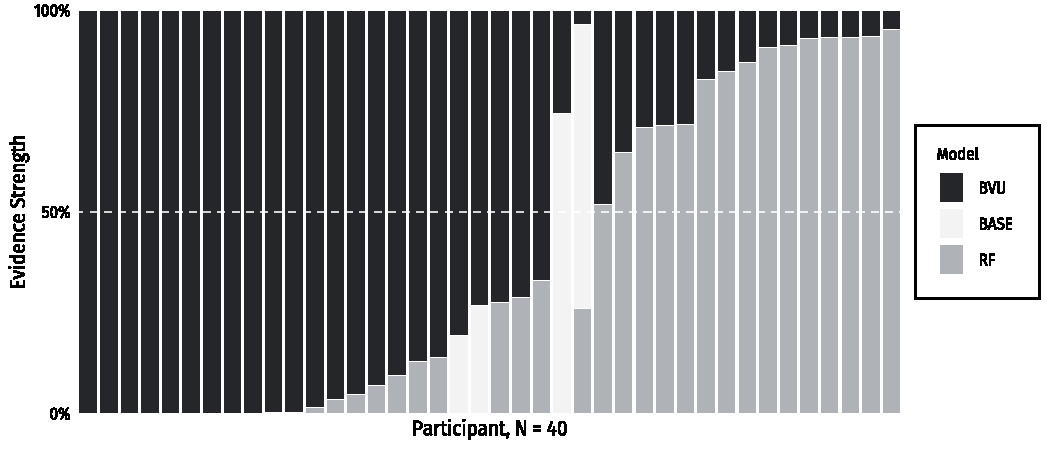
\includegraphics[width=.9\linewidth]{../figures/fig2-1} 

}

\caption{Evidence for the models for individual participants. \textit{RF}$=$ relative frequency model, \textit{BVU}$=$ Bayesian value updating model, \textit{BASE}$=$ Baseline model.}\label{fig:fig2}
\end{figure}

\added[id=jj]{
The fitted model parameters (Table \ref{tab:study1_parameter}) reveal that the power utility exponent did not differ markedly between the participants that were described by the Bayesian value updating strategy ($M_{\alpha}= 2.19$) and those described by a relative frequency strategy ($M_{\alpha}=2.15$), $\Delta$ $M = 0.04$ 95\% HDI $[-1.07$, $1.18]$, $\mathrm{BF}_{\textrm{01}} = 3.21$. Participants using the Bayesian strategy had, on average, a prior belief that gains occur with 45\% (gain prior $\theta_G = 0.91$; zero-outcome prior $\theta_0 = 1.09$). Also, their estimated learning rate $\delta$ was anti-conservative ($M_{\delta}=2.27$).
}

\begin{table}[tbp]

\begin{center}
\begin{threeparttable}

\caption{\label{tab:study1_parameter}Parameter Estimates of Winning Models, \textit{M (SD)}}

\begin{tabular}{lcccc}
\toprule
Winning Model & $\alpha$ & $\delta$ & $\theta_G$ & $\sigma$\\
\midrule
BVU (\textit{n}$=$23) & 2.19 (2.35) & 2.27 (3.39) & 0.91 (0.79) & 0.23 (0.22)\\
RF (\textit{n}$=$17) & 2.15 (1.45) & -- & -- & 0.15 (0.04)\\
\bottomrule
\addlinespace
\end{tabular}

\begin{tablenotes}[para]
\normalsize{\textit{Note.} \textit{BVU}$=$ Bayesian value updating model, \textit{RF}$=$ relative frequency model. Parameters denote: $\alpha=$ power utility exponent, $\theta_G$ gain prior, $\sigma$ standard deviation.}
\end{tablenotes}

\end{threeparttable}
\end{center}

\end{table}

\textit{Qualitative Model Fit.} Figure \ref{fig:fig5} plots the
qualitative model fit (best-fitting model predictions against observed
evaluations by participant). As in Study 1, the data are generally
well-described
\added[id=jj]{($M r\textsubscript{pred,obs} = 0.70$), except in four cases (participants s42, s47, s54, s67, with $r\textsubscript{pred,obs} < 0.40$)}
where the model must be rejected because of qualitative mis-fit.

\begin{figure}[htb]

{\centering 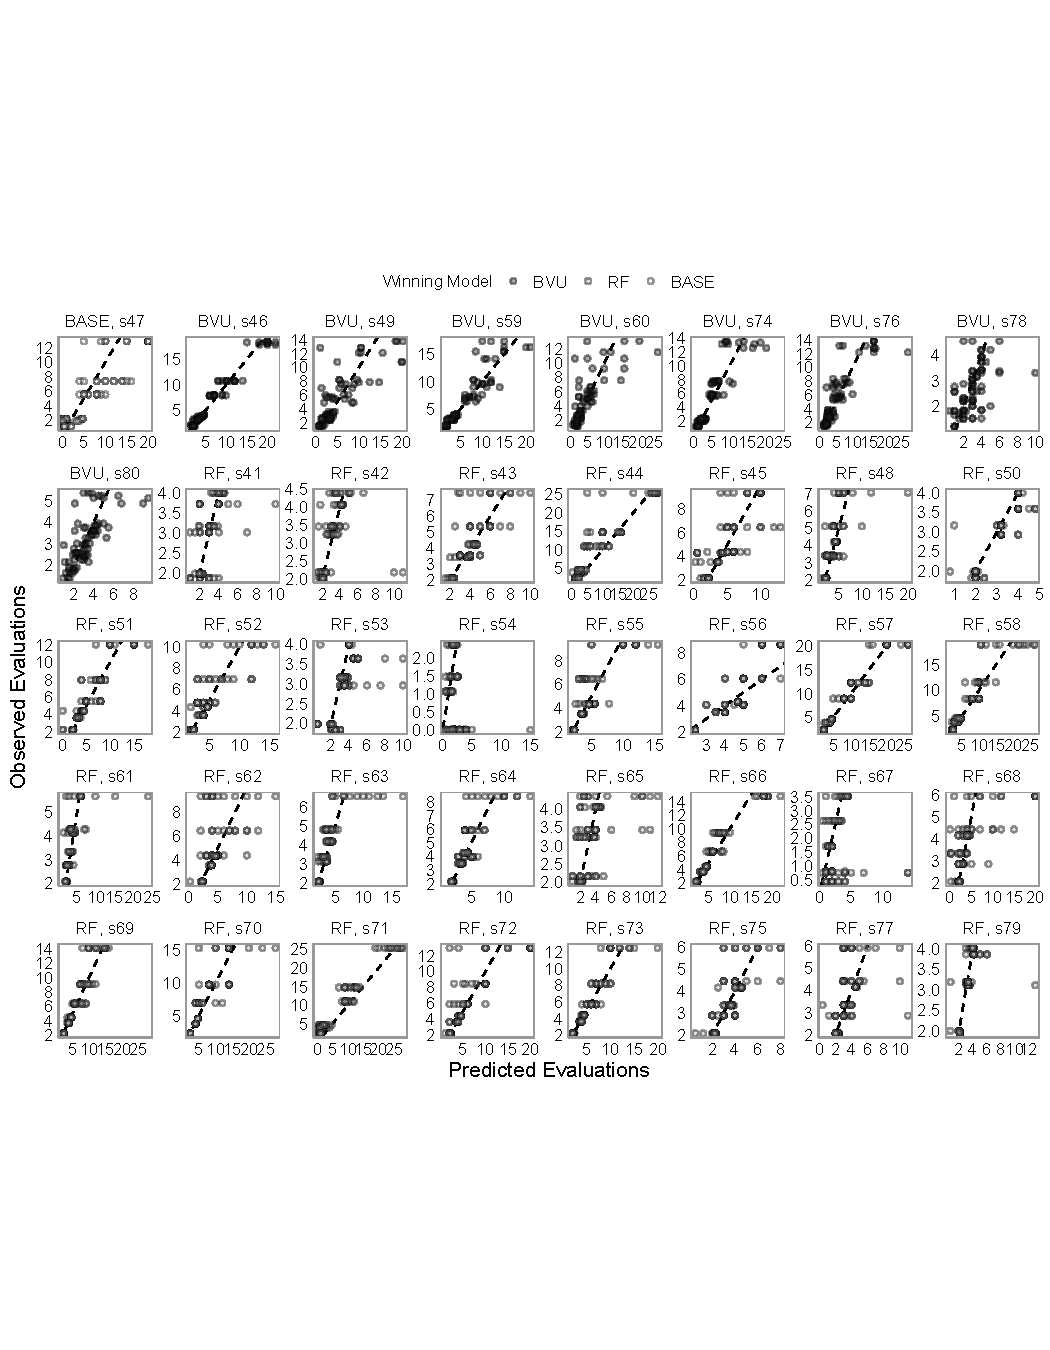
\includegraphics[width=.9\linewidth]{../figures/fig5-1} 

}

\caption{Predicted evaluations from the best-fitting models plotted against the observed evaluations (by participant). \textit{BVU}$=$ Bayesian value updating model, \textit{RF}$=$ relative frequency model.}\label{fig:fig5}
\end{figure}


\end{document}

\clearpage

\subsection{Discussion of Study 2}
Study 2 tested whether the results of Study 1  generalize to typical sampling paradigms where people learn the outcome values from experience. The results of Studies 1 and 2 are very similar: participants mean evaluations were not influenced by sample size systematically, and in line with Study 1, we found that a substantial proportion of people could be classified as Bayesian learners. In Study 2, however, a greater proportion of participants was described by a \added[id=jj]{potentially cognitively simpler} relative-frequency-based cognitive model.

\clearpage %forces figures and tables to be printed HERE

\section{Test of Qualitative Predictions from the Cognitive Models}
\added[id=jj]{The next analyses examine qualitative predictions from the Bayesian value updating and the relative-frequency model of learning probabilities. We pooled the observed data from both studies (N= 80) and classified participants by the best-fitting models from the cognitive modeling results.}


\textit{Predictions about gamble valuations.}
\added[id=jj]{Regarding the valuations, the relative frequency model predicts no effect of sample size on valuations in our task (because the relative frequencies did not differ across sample sizes). In contrast, the Bayesian value updating model predicts that given different prior beliefs the frequency of experienced outcomes will change people's beliefs in different directions, and that this change is stronger with larger sample size (Figure~ \ref{fig:sensi}). According to the Bayesian value updating model, participants with a prior belief that zero outcomes are more likely than gain outcomes (zero-outcome prior) who sample p-bets should increase their evaluations with higher sample size. By contrast, participants with a prior belief that gains are more likely than zero outcomes (gain prior) who sample \$-bets should decrease their valuations with higher sample size.}

\documentclass[a4paper, man, floatsintext]{apa6}
\usepackage{lmodern}
\usepackage{amssymb,amsmath}
\usepackage{ifxetex,ifluatex}
\usepackage{fixltx2e} % provides \textsubscript
\ifnum 0\ifxetex 1\fi\ifluatex 1\fi=0 % if pdftex
  \usepackage[T1]{fontenc}
  \usepackage[utf8]{inputenc}
\else % if luatex or xelatex
  \ifxetex
    \usepackage{mathspec}
  \else
    \usepackage{fontspec}
  \fi
  \defaultfontfeatures{Ligatures=TeX,Scale=MatchLowercase}
\fi
% use upquote if available, for straight quotes in verbatim environments
\IfFileExists{upquote.sty}{\usepackage{upquote}}{}
% use microtype if available
\IfFileExists{microtype.sty}{%
\usepackage{microtype}
\UseMicrotypeSet[protrusion]{basicmath} % disable protrusion for tt fonts
}{}
\usepackage{hyperref}
\hypersetup{unicode=true,
            pdfauthor={Jana B. Jarecki},
            pdfborder={0 0 0},
            breaklinks=true}
\urlstyle{same}  % don't use monospace font for urls
\usepackage{graphicx,grffile}
\makeatletter
\def\maxwidth{\ifdim\Gin@nat@width>\linewidth\linewidth\else\Gin@nat@width\fi}
\def\maxheight{\ifdim\Gin@nat@height>\textheight\textheight\else\Gin@nat@height\fi}
\makeatother
% Scale images if necessary, so that they will not overflow the page
% margins by default, and it is still possible to overwrite the defaults
% using explicit options in \includegraphics[width, height, ...]{}
\setkeys{Gin}{width=\maxwidth,height=\maxheight,keepaspectratio}
\IfFileExists{parskip.sty}{%
\usepackage{parskip}
}{% else
\setlength{\parindent}{0pt}
\setlength{\parskip}{6pt plus 2pt minus 1pt}
}
\setlength{\emergencystretch}{3em}  % prevent overfull lines
\providecommand{\tightlist}{%
  \setlength{\itemsep}{0pt}\setlength{\parskip}{0pt}}
\setcounter{secnumdepth}{0}
% Redefines (sub)paragraphs to behave more like sections
\ifx\paragraph\undefined\else
\let\oldparagraph\paragraph
\renewcommand{\paragraph}[1]{\oldparagraph{#1}\mbox{}}
\fi
\ifx\subparagraph\undefined\else
\let\oldsubparagraph\subparagraph
\renewcommand{\subparagraph}[1]{\oldsubparagraph{#1}\mbox{}}
\fi

%%% Use protect on footnotes to avoid problems with footnotes in titles
\let\rmarkdownfootnote\footnote%
\def\footnote{\protect\rmarkdownfootnote}

%%% Change title format to be more compact
\usepackage{titling}

% Create subtitle command for use in maketitle
\providecommand{\subtitle}[1]{
  \posttitle{
    \begin{center}\large#1\end{center}
    }
}

\setlength{\droptitle}{-2em}

  \title{}
    \pretitle{\vspace{\droptitle}}
  \posttitle{}
    \author{Jana B. Jarecki}
    \preauthor{\centering\large\emph}
  \postauthor{\par}
      \predate{\centering\large\emph}
  \postdate{\par}
    \date{15 Januar, 2020}

\usepackage{natbib} \usepackage{threeparttable} \usepackage{booktabs}
\shorttitle{test} \usepackage{setspace}
\AtBeginEnvironment{tabular}{\singlespacing} \usepackage{times}
\usepackage{changes} \definechangesauthor[name={JJ}, color=orange]{jj}
\usepackage{upgreek} \AtBeginDocument{\let\maketitle\relax}

\begin{document}

\added[id=jj]{To test these hypotheses, Participants were classified as relative-frequency learners (RF-type; $n=25$), Bayesian learners with prior beliefs that gains are more likely than zero outcomes, $\alpha_0 > \beta_0$ ($n=14$), and Bayesian learners with prior beliefs that zero outcomes are more likely than gains, $\alpha_0 < \beta_0$ ($n=32$), based on the individually best-fitting cognitive model. The participants that were best described by the baseline model and that showed qualitative model mis-fit (Figures \ref{fig:fig3} and \ref{fig:fig5}) were excluded ($n=9$).}

\added[id=jj]{Figure \ref{fig:fig6}a shows that the RF-type participants kept their valuations relatively stable independent of sample size whereas the Bayesian participants changed their evaluations with sample size. Those Bayesian participants who were described by a prior belief that zero outcomes were very likely (zero-outcome prior) increased their evaluations of p-bets. Those Bayesian participants who were described by prior belief that positive outcomes were very likely (gain prior) slightly decreased their evaluations of \$-bets, as predicted. Statistical analyses by means of a Bayesian mixed-effects model}\footnote{Regressing the (normalized, within-person z-standardized) evaluations on the predictors sample size category (coded as 1,2,3,4), gamble type, and learner class (BVU-gain-prior, BVU-loss-prior, RF) and interactions of the predictors, with a by-participant random intercept; categorical predictors were effects-coded to facilitate interpretation of interactions. The statistical model used weakly informative priors.}
\added[id=jj]{supported a model that includes a sample size x learner type interaction and a gamble type x learner type interaction ($M_1$) over a model without the first interaction term ($BF\textsubscript{10} = 12$) and over a model without the second interaction term ($BF\textsubscript{20} > 1000$). The modal posterior regression coefficient estimates for the effect of sample size on valuation in Bayesian learners with zero-outcome priors who sampled p-bets was positive, $b_\textsubscript{BVU,zero,p-bet}$ $=0.14$ (89\% HDI $0.11, 0.18$), and for Bayesians with gain priors who sampled \$-bets the estimate was negative, $b_\textsubscript{BVU,gain,\$-bet}$ $=-0.01$ (89\% HDI $-0.09, 0.00$), as hypothesized. For RF-type participants and contrary to the RF model predictions, the estimated regression coefficients for the effect of sample size on the valuations showed trends: the modal coefficient for p-bets was $b_\textsubscript{RF,p-bet}$ $=-0.00$ (89\% HDI $-0.08, -0.00$), and for \$-bets it was $b_\textsubscript{RF,\$-bet}$ $=0.05$ (89\% HDI $0.04, 0.12$). This indicates that even those participants best-described by the relative frequency model were influenced by sample size to a small degree.}

\begin{figure}[htb]

{\centering 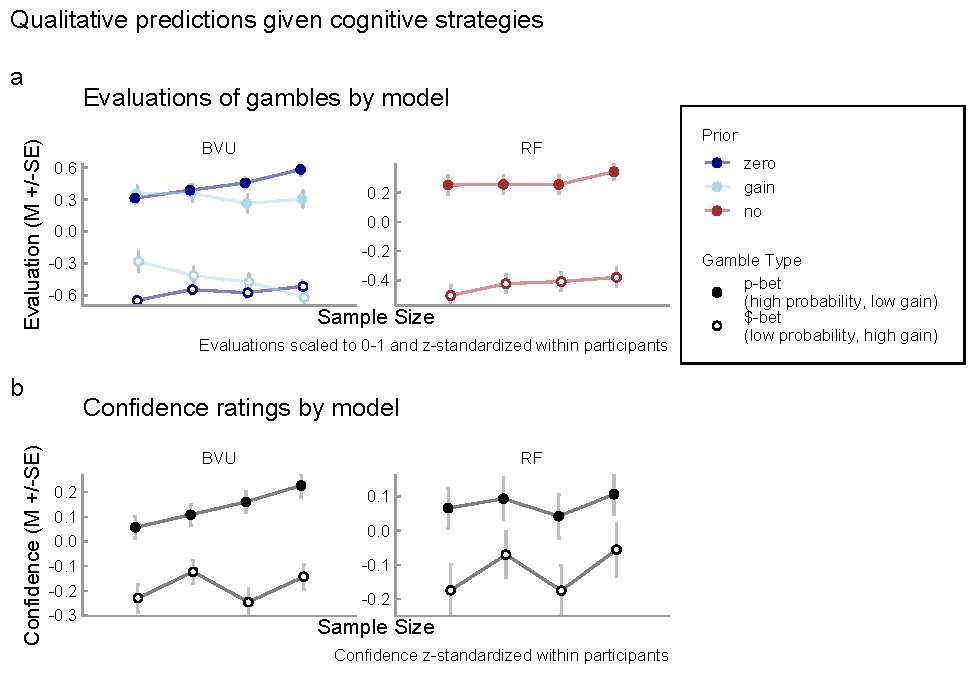
\includegraphics[width=.9\linewidth]{../figures/fig6-1} 

}

\caption{Mean evaluations by gamble type and best-fitting cognitive model and prior beliefs of the BVU model. \textit{BVU}$=$Bayesian value updating model, \textit{RF}$=$ Relative frequency model. Error bars indicate standard errors. Sample size categories see Table \ref{table:Lotteries}. Evaluations are scaled to 0-1 and z-standardized at the individual level.}\label{fig:fig6}
\end{figure}

\textit{Predictions about confidence.}
\added[id=jj]{The Bayesian model also predicts that people's confidence in their beliefs should increase with more evidence they gather. Thus Bayesian learners' confidence is expected to increase with sample size. The relative frequency model makes no predictions about confidence. To test this, we classified participants into Bayesian and relative-frequency learners based on the best-fitting model. Mean confidence ratings of Bayesian-type learners, z-standardized within participants, increased only slightly from the extra small sample size ($M=-0.07, SD=1.00$), to the small sample size ($M=0.01, SD=0.91$), medium sample size ($M=-0.01, SD=1.00$), and large sample size ($M=0.07, SD=1.00$, Figure \ref{fig:fig6}b), but statistical analyses showed that a linear regression model}\footnote{Regressing the (within-person z-standardized) confidence ratings on the predictors sample size category (coded as 1,2,3,4), gamble type, and winning model (BVU, RF), and interactions of the predictors, with a by-participant random intercept; categorical predictors were effects-coded to facilitate interpretation of interactions.}
\added[id=jj]{($M_1$) that includes the sample size as predictor performed worse than an intercept-only model ($BF_{01}> 1000$).}


\end{document}


\textit{Discussion of the qualitative cognitive model predictions.}
\added[id=jj]{Learners that seemed to follow a Bayesian strategy changed their evaluations in line with Bayesian principles, but also the learners that followed a relative frequency strategy showed slight changes in evaluations with sample size. Regarding the influence of sample size on confidence ratings, the Bayesian model's prediction of growing confidence with growing sample size received no support.}

\section{General Discussion}
A number of studies have shown that the amount of experience people gain with the outcome distribution of risky options affects risk preferences and risky choice. We manipulated the amount of experience (sample size) with risky options to investigate specifically, how the sample size influences risk preferences and evaluations in the gain domain.

\added[id=jj]{Study 1 consisted of an experience-based sampling task in which participants were informed about the outcomes of two binary risky options. By sampling outcomes participants learned about the probabilities with which outcomes occurred. To examine the effect of experience on people's evaluation of risky gambles we manipulated the sample size of outcomes participants drew within-subject. The samples were predetermined so that the relative frequencies of the samples were representative of the expected value, which allowed us to control for sampling errors and isolate the mere effects of sample size on judgments. We tested whether participants' evaluation could be best predicted by a relative frequency (RF) model, that essentially ignores sample size, or a Bayesian value updating (BVU) model, that takes sample size into account. Most participants' evaluations were best described by the BVU model with an initial prior belief that the zero outcome occured with a larger probability than the positive gain outcome. These prior belief were however quickly overcome by learning from experience. Only around a quarter of participants were best-described by the RF model. Participants' confidence in evaluations, however, were not substantially affected by sample sizes.}

\added[id=jj]{Study 2 was quite similar to Study 1, with the only difference that the potential outcomes of the risky options were not told to the participants before sampling outcomes. Therefore the potential outcomes had to be learned during the sampling process. Again, the size of the samples that participants drew was manipulated. The results are in line with Study 1: while mean evaluations and confidence were largely unaffected by the sample size manipulation, cognitive modeling results showed that a Bayesian strategy described the behavior of slightly more than half of participants well (57\%) and that the learners had an initial belief that the zero outcome was more likely than the positive outcome, which they updated fast through sampling.}

\added[id=jj]{The relative frequency model described a minority of participants best in both studies. This finding is in line with previous results suggesting that people often believe in the representativeness of short sequences of outcomes \citep{Griffin1992, Tversky1971}. This could also explain why people in experience-based tasks often do not sample much: If people believe that a short sequence of outcomes represents a prospect's outcome distribution comprehensively, they do not need to sample much, as they believe that sampling more will not yield new information.}

Our results suggests a substantial degree of heterogeneity of how people sample information and integrate the observed information for a final judgment. It is an open question why some of our participants behaved according to Bayesian principles and others did not. Thus, future research is needed to examining what factors influence whether people behave according to Bayesian principles. One possible candidate that mediates what strategy people use could be numerical literacy, which has been shown in previous work to be related to performance in Bayesian reasoning tasks \citep{Brase2017}.

\subsubsection{The role of prior beliefs}
\added[id=jj]{The Bayesian model assumes that people start sampling with an initial belief about the probabilities of different outcomes. Our data suggest that most Bayesian learners started with the prior belief that the zero-outcome was quite likely, but this belief was then quickly overruled by incoming experience. In contrast to previous work, which has indicated that people are slow Bayesian updaters, we find that people update quicker than optimal Bayesian with a liberal learning rate.}

We have assumed that over the course of the experiment and across different gambles, people's prior beliefs do not change. However, recent research suggests that knowing the gain amount elicits a more informed prior belief about the probability. Under uncertainty, people's beliefs about gain probabilities are informed by the gain amount: Large gains are believed to be less likely than small gains when no other information about a gamble than the gain amount is given \citep{Pleskac2014, Hoffart2018}. If in our studies people indeed used gain amounts as predictors of the probability and integrated this information with their samples, this can explain why we see only a small effect of sample size on gamble valuations. This is because in our experimental design large gains were indeed less likely than small gains. Thus, it corresponded to the probability--reward pattern that people might presuppose. If people start sampling with prior probability beliefs that correspond closely to the real outcome probabilities, new incoming information does not shift probability beliefs as dramatically as when the prior beliefs are uninformed (e.g., uniform priors). Future research could investigate this hypothesis, for instance, by investigation how sample size influences valuations in \textit{nonrepresentative} environments, such as environments where the size of a reward/gain is uncorrelated with the probability that it occurs.

\subsection{Description versus experience in choice and valuation}
\added[id=jj]{Study 1's findings differ from the classic description-experience gap, that is the  participants did not behave as if they overweight rare events from description and underweight rare events from experience. In the valuation tasks participants behaved as if they overweighted rare events from both description and experience, when they were informed about the outcomes before sampling.}
Importantly, in contrast to standard experience-based choice tasks where participants experience two lotteries and make binary choices, the participants had to evaluate one individual gamble in each trial. \cite{Lichtenstein1971}, for instance, report preference reversals when people evaluate rather than chose options (a person who chooses Gamble A over Gamble B may assign a higher value to Gamble B than to Gamble A). Our valuation data is not in line with other work on evaluations from experience, that finds stronger over-weighting of rare events in an experience- than a description-format \citep{Golan2014}, but this design differs from our task in that it did not use representative outcome sequences. As we argued in the Introduction, in free-sampling paradigms, the experienced relative frequencies of outcomes do not necessarily match the underlying probability and the resulting sampling error might have contributed to the difference in the results. It is further conceivable that people show different information processing in free- and forced-sampling paradigms. For instance, people may pay more attention to a voluntarily sampled outcome than to a sampled outcome that resulted from a forced sampling decision.

\subsubsection{Buying versus selling prices}
In both studies participants were asked for their selling prices of the gambles to elicit people's preferences. The endowment effect describes that people attach higher value to goods when they sell them than when they buy them \citep{Thaler1980}. \cite{Pachur2012} demonstrated this endowment effect in an experience-based task. It would be interesting to replicate our experiments with buying instead of selling prices and more rigorously compare the results with buying and selling prices from description. However, this was beyond the scope of the present study. Here, our main focus was to investigate whether preferences are influenced by sample sizes. This question can be answered independently of response format. Irrespective of whether people are asked for selling prices or buying prices or make repeated choices, the Bayesian model predicts an effect of sample size on valuations. 

\subsubsection{Confidence in valuations from description and experience}
People were more confident with their gamble valuations from experience than from description. This finding is remarkable given that from a normative perspective one could argue that people feel more confident when making valuations from description than when making valuations from experience. This is because valuations from description do not entail any uncertainty about the outcome distributions, whereas valuations from experience may entail such uncertainty.

Our findings do support research by \cite{Bradbury2014}. They reported that people who made investment decisions in the laboratory felt better informed and were more confident about their decisions from experience than those from description.
Potentially, people perceive and process experienced information differently from described information \citep{Kahneman2009}: 
While information that is described is more abstract, experienced information has direct salience or impact. When people draw a sample, they not only observe the outcome but also experience emotional reactions resulting from that observation. Thus, people do not only learn plain facts about the outcome distribution; they also gain a more vivid understanding of this distribution. This more concrete understanding of the risky option can help people access their preferences and thus creates higher confidence in valuations.


\bibliography{refJanine,references}

%\section{Footnotes}



%Kahnemann (2009): In fact, people are poor forecasters of their future emotions and future tastes—they need help in this task—and I believe that one of the responsibilities offinancial advisors should be to pro-vide that help.

\end{document}


% Please see the package documentation for more information
% on the APA6 document class:
%
% http://www.ctan.org/pkg/apa6
%